\chapter{实验结果与评估}
\label{chap:4}
本章主要对第三章提出的模型，即融合物理信息的基于Swin Transformer双分支预测模型，进行实验验证与性能评估。首先介绍实验的数据集划分策略、硬件环境与超参数设置；其次通过合理的评价指标验证模型在野火预测任务上的整体表现；最后，通过消融实验（Ablation Study）深入剖析各核心物理模块的有效性。
\section{数据集预处理及实验设置}
\label{sec:4-1}
考虑到野火发生具有强烈的季节性与气候周期性规律，为避免未来数据泄露到历史训练中，本实验参考\cite{loan}，采用基于时间序列的划分准则。将数据集中 2019 年之前的历史火灾与非火灾样本划分为训练集（Training Set），用于模型参数的优化；2019 年的全年样本作为验证集（Validation Set），用于监控训练过程并进行早停（Early Stopping）等决策；2020 年与 2021 年的数据作为相互独立的测试集（Test Set），用于评估模型在未知未来年份上的泛化性能。

在数据输入网络前，对所有连续型气象特征执行了全局最大最小值归一化（Min-Max Normalization），将其线性映射至 $[0, 1]$ 区间，以消除不同气象要素（如风速、温度）量纲差异对梯度反向传播的干扰。针对真实遥感与气象数据中存在的异常或缺失值，采用零填充策略处理。同时，设定动态气象变量的时间窗口步长为 10 天，即模型基于起火日前连续 10 天的气象序列进行预测。

本研究的所有深度学习模型均基于 PyTorch（2.5.1 版本）框架开发。在硬件配置方面，模型的训练与推理计算使用2张NVIDIA GeForce RTX 4080（32GB显存）。

由于本任务属于正负样本不平衡的时空二分类问题，因此在训练集加载阶段启用了数据增强（Data Augmentation）机制，如水平翻转和垂直翻转等，以扩充样本多样性，并保持正负样本比例为1：2\cite{loan}。在损失函数与激活函数的选取上，本实验在分类头末端采用 LogSoftmax 激活函数将输出映射为对数概率，并选用加权负对数似然损失函数（Weighted NLLLoss）进行模型优化。考虑到模型训练初期的梯度稳定性，本研究在基线训练阶段对非火灾样本（负类）与火灾样本（正类）赋予了均等的损失权重（$[0.5, 0.5]$），以确保模型优先学习大尺度下的基础时空气象映射规律。

在优化算法方面，选用适配 Transformer 架构的 AdamW 优化器，以利用其权重衰减（Weight Decay）特性防止过拟合，半权重衰减系数设定为 0.03，并结合丢弃率（Dropout Rate）为 0.3 的随机失活策略。初始学习率设定为 $3 \times 10^{-5}$，并配合阶梯式学习率调度策略（StepLR），每 12 个 Epoch 将学习率衰减至原来的 10\%，使模型在训练后期能够持续梯度下降。模型训练的批次大小（Batch Size）设定为 256，总训练轮次（Epoch）设定为 40 轮。

\section{实验设置与评价指标}
\label{sec:4-2}

\subsection{实验组别设置}
为了验证本研究\ref{sec:3-5}提出的物理启发——基于热力学先验的饱和水汽压差和风场矢量作为动力学偏置注入注意力网络——在野火预测任务中的有效性，设计了以下四组对比实验：

\begin{enumerate}
    \item[(1)] \textbf{基础双分支网络 (Baseline)}：剥离物理先验模块，使用动态气象特征与静态地貌特征输入 2D/3D Swin Transformer 双分支网络进行特征提取与分类。
    \item[(2)] \textbf{引入热力学特征的网络 (+VPD)}：在 Baseline 的基础上，利用马格努斯-泰登经验公式将基础气象数据重构为饱和水汽压差（VPD），也作为动态变量输入网络，以强化模型对火灾易发干旱环境的感知。
    \item[(3)] \textbf{引入动力学偏置的网络 (+UV)}：在 Baseline 的基础上，在特征融合阶段的地理感知交叉注意力机制（Geo-CA）中，将风场的经向速度 U、纬向速度V分量作为空间偏置（Spatial Bias）注入网络，引导模型关注风向带来的火势蔓延趋势。
    \item[(4)] \textbf{物理融合网络 ( +VPD \& +UV)}：本研究提出的最终模型架构，同时融合 VPD 热力学特征重构与 Geo-CA 风场动力学偏置，实现物理信息与数据驱动的深度结合。
\end{enumerate}
\subsection{评估指标}
野火预测本质上是基于极度不平衡数据的时空二分类任务。为全面客观地评估模型的性能，本实验按照前述研究的评估方法\cite{loan,dacsa,kondylatos2022wildfire}，引入混淆矩阵（Confusion Matrix），包括真正例（TP, True Positive）、假正例（FP, False Positive）、真负例（TN, True Negative）和假负例（FN, False Negative）。在此基础上，选取五项评价指标：

\begin{itemize}
    \item \textbf{精确率 (Precision)}：在模型所有预测为有火的样本中，真正有火的比例。体现了预测的准度，数值越高代表误报率越低。
    $$ Precision = \frac{TP}{TP + FP} $$
    
    \item \textbf{召回率 (Recall)}：在实际真正有火的样本中，模型成功预测出来的比例。体现了预测的全度，数值越高代表漏报率越低。在野火防灾业务中，漏报的代价远高于误报，因此该指标极具参考价值。
    $$ Recall = \frac{TP}{TP + FN} $$
    
    \item \textbf{F1 分数 (F1-Score)}：精确率与召回率的调和平均数。由于野火非着火背景极多，F1-Score 能够更好地衡量模型的综合性能。
    $$ F1\text{-}Score = 2 \times \frac{Precision \times Recall}{Precision + Recall} $$
    
    \item \textbf{AUROC (Area Under the ROC Curve)}：指受试者工作特征曲线（ROC）下的面积。它衡量了模型在不同分类判定阈值下，区分正负样本的综合能力，数值越接近 1 代表模型的区分能力越强。在数学上等价于，模型随机抽取一个正样本和负样本，正样本的预测概率排在负样本之前的概率：
    $$ AUROC = \frac{\sum_{i \in \mathcal{P}} \sum_{j \in \mathcal{N}} \mathbb{I}(p_i > p_j)}{|\mathcal{P}| \times |\mathcal{N}|} $$
    其中，$\mathcal{P}$ 和 $\mathcal{N}$ 分别为真实的正类（有火）与负类（无火）样本集合，$p_i$ 与 $p_j$ 代表模型输出的预测概率，$\mathbb{I}(\cdot)$ 为指示函数，当括号内条件成立时，指示函数值为 1，否则为 0。该公式证明了 AUROC 不受极端正负样本比例失衡的影响，也是评估野火预测模型的关键指标。
    \item \textbf{总体准确率 (Overall Accuracy, OA)}：模型正确预测的样本（含正类与负类）占总样本的比例，反映模型的整体预测正确度。
    $$ OA = \frac{TP + TN}{TP + TN + FP + FN} $$
    
\end{itemize}

\subsection{模型训练与收敛性验证}
为验证模型在训练过程中的稳定性，图\ref{fig:4-2-train_val_loss}展示了模型在训练集与验证集上的损失（Loss）演变曲线，分别是基础模型与加入不同物理信息启发的模型。可以看出，随着迭代轮次（Epoch）的增加，训练集与验证集的损失曲线在前期快速下降，之后逐渐进入平稳收敛区。
\begin{figure}[htbp]
    \centering
    % 左图：Loss 曲线
    \begin{minipage}{0.48\textwidth}
        \centering
        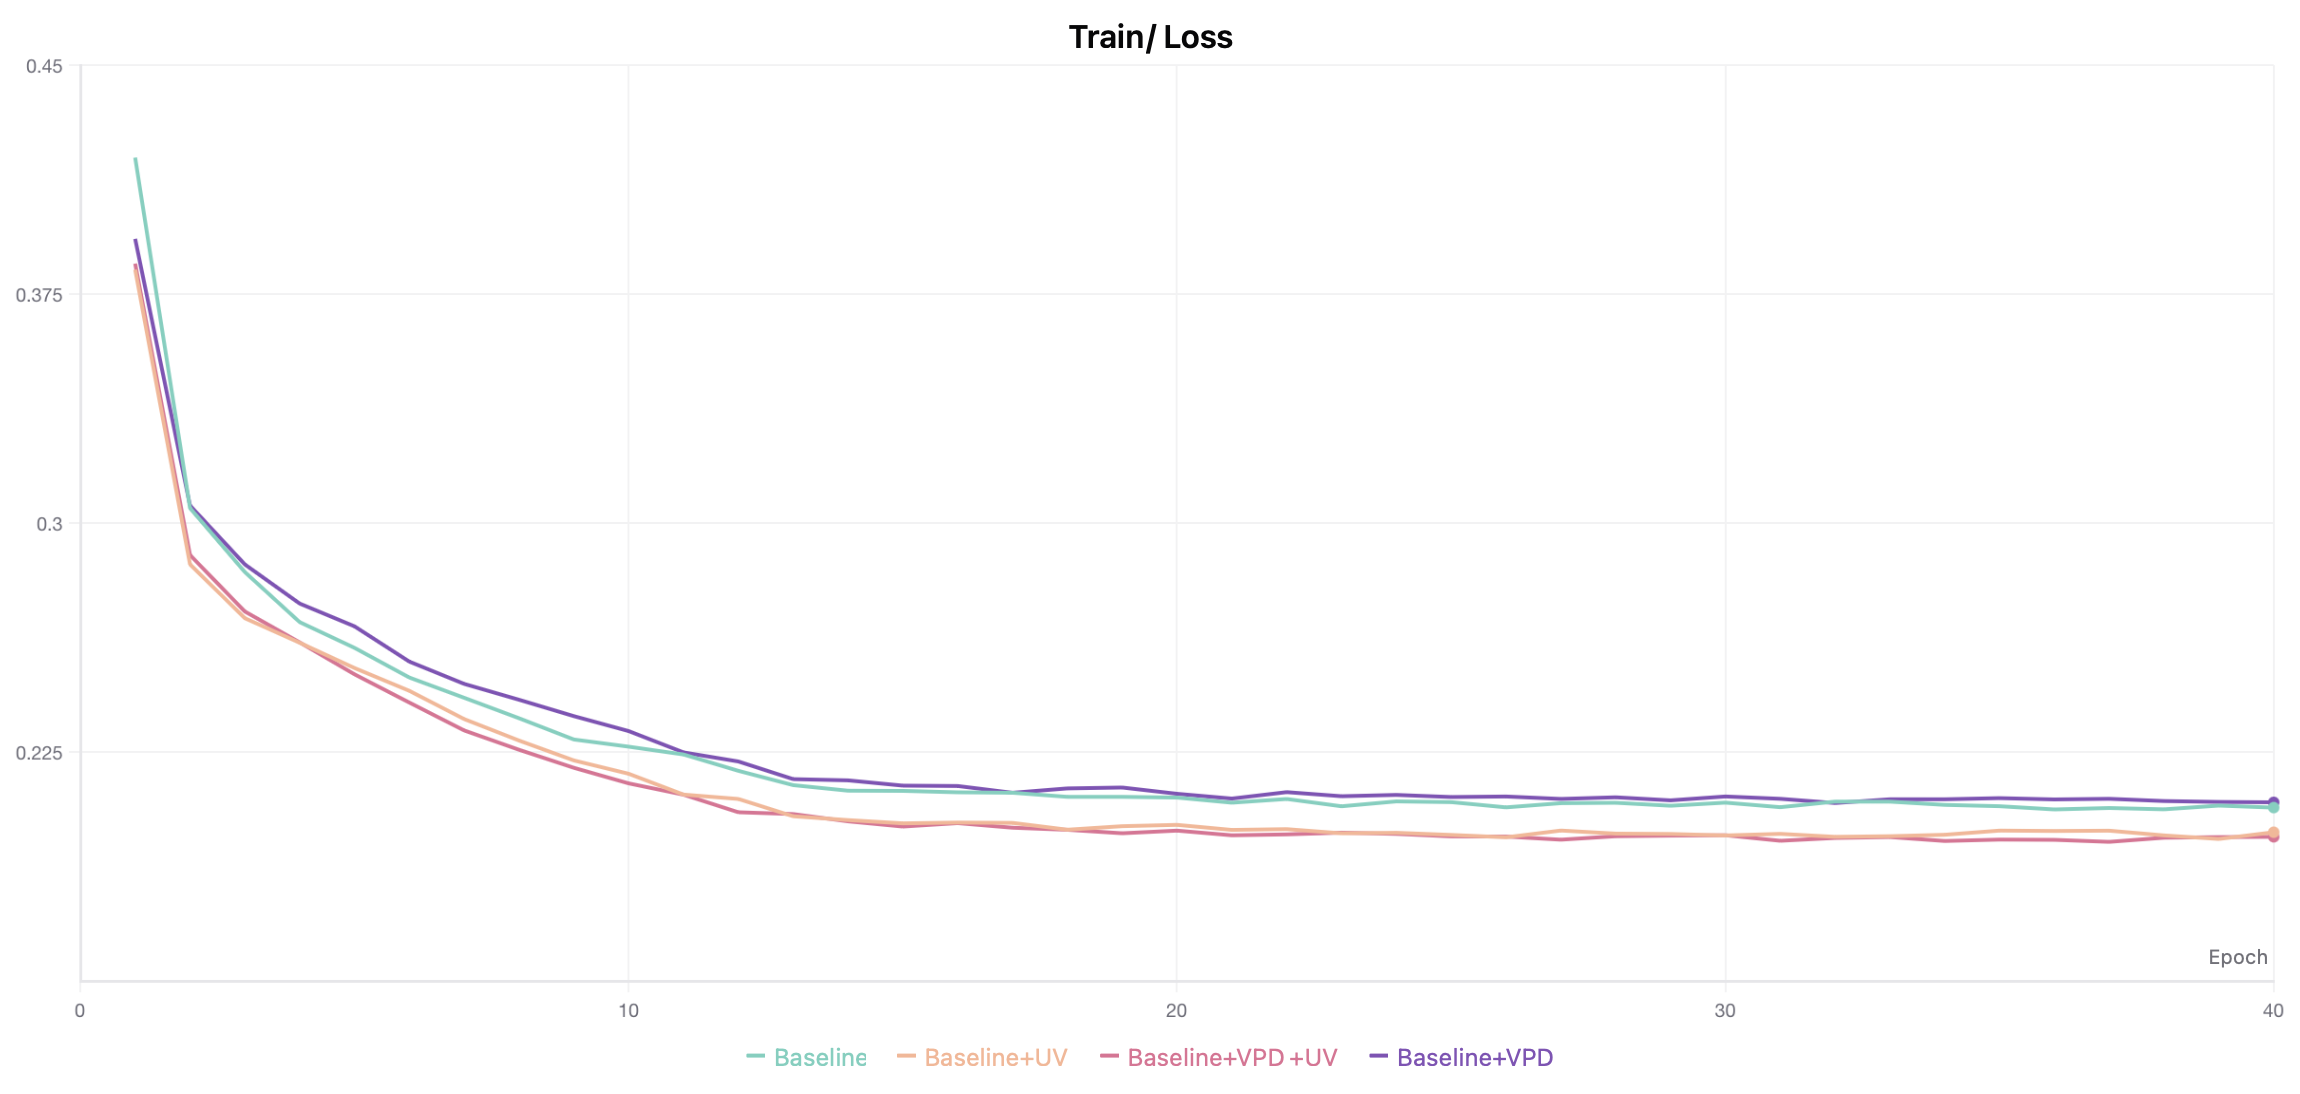
\includegraphics[width=\linewidth]{img/chap4/4-2-train-loss.png} 
        \centerline{(a) 训练集 Loss 曲线}
    \end{minipage}\hfill
    % 右图：Precision 曲线
    \begin{minipage}{0.48\textwidth}
        \centering
        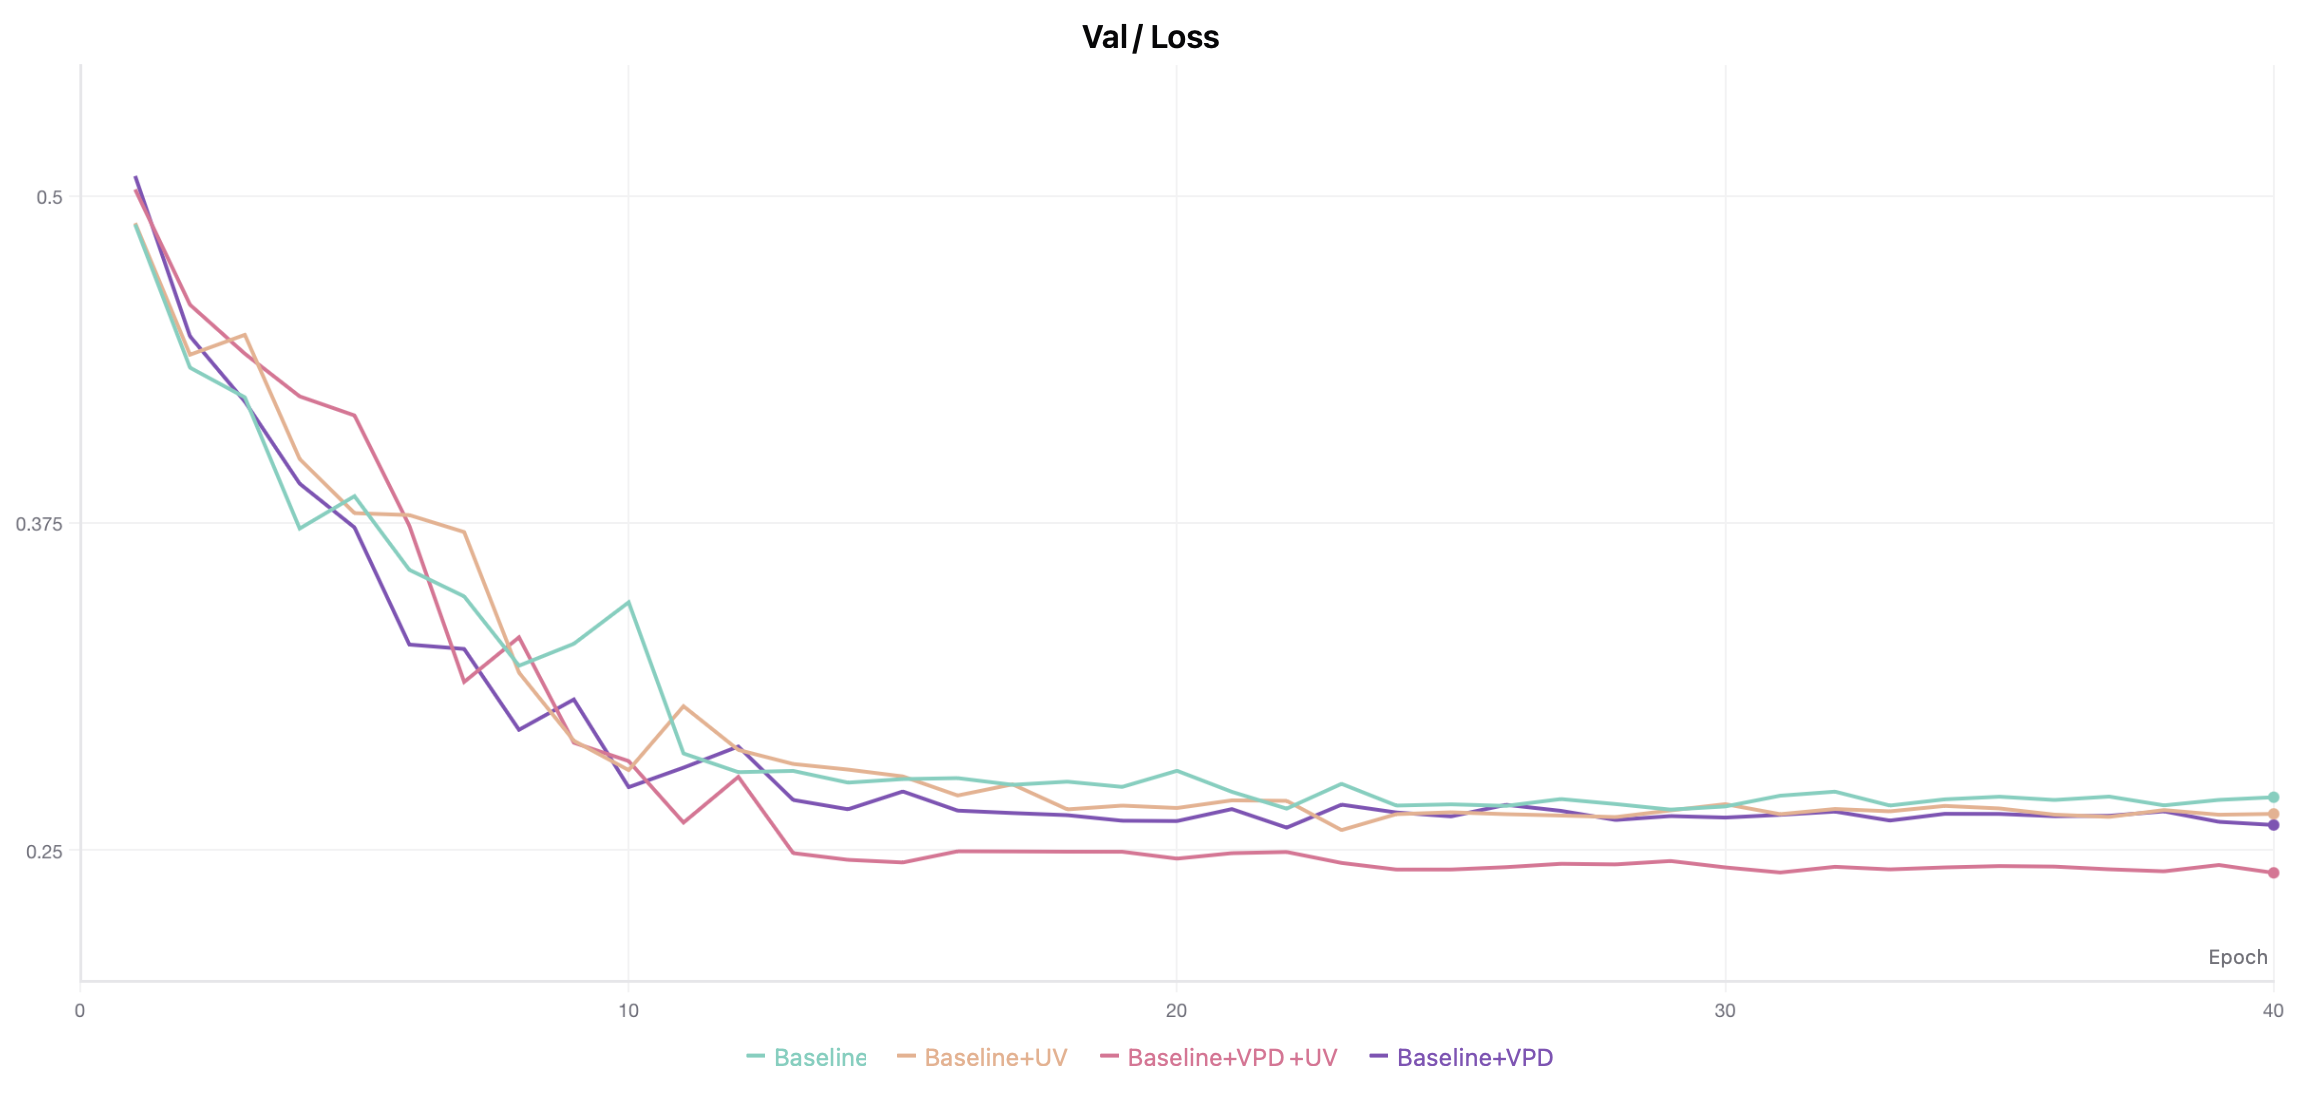
\includegraphics[width=\linewidth]{img/chap4/4-2-val-loss.png} % 替换为你的precision图路径
        \centerline{(b) 验证集 Loss 曲线}
    \end{minipage}
    \caption{模型训练过程中的Loss曲线}
    \label{fig:4-2-train_val_loss}
\end{figure}

同时，图 \ref{fig:4-2-train_val_precision}展示了模型训练过程中的精确率（Precision）曲线，表明模型的查准能力随着训练得到稳步提升，最终收敛于高置信度区间。
\begin{figure}[htbp]
    \centering
    \begin{minipage}{0.48\textwidth}
        \centering
        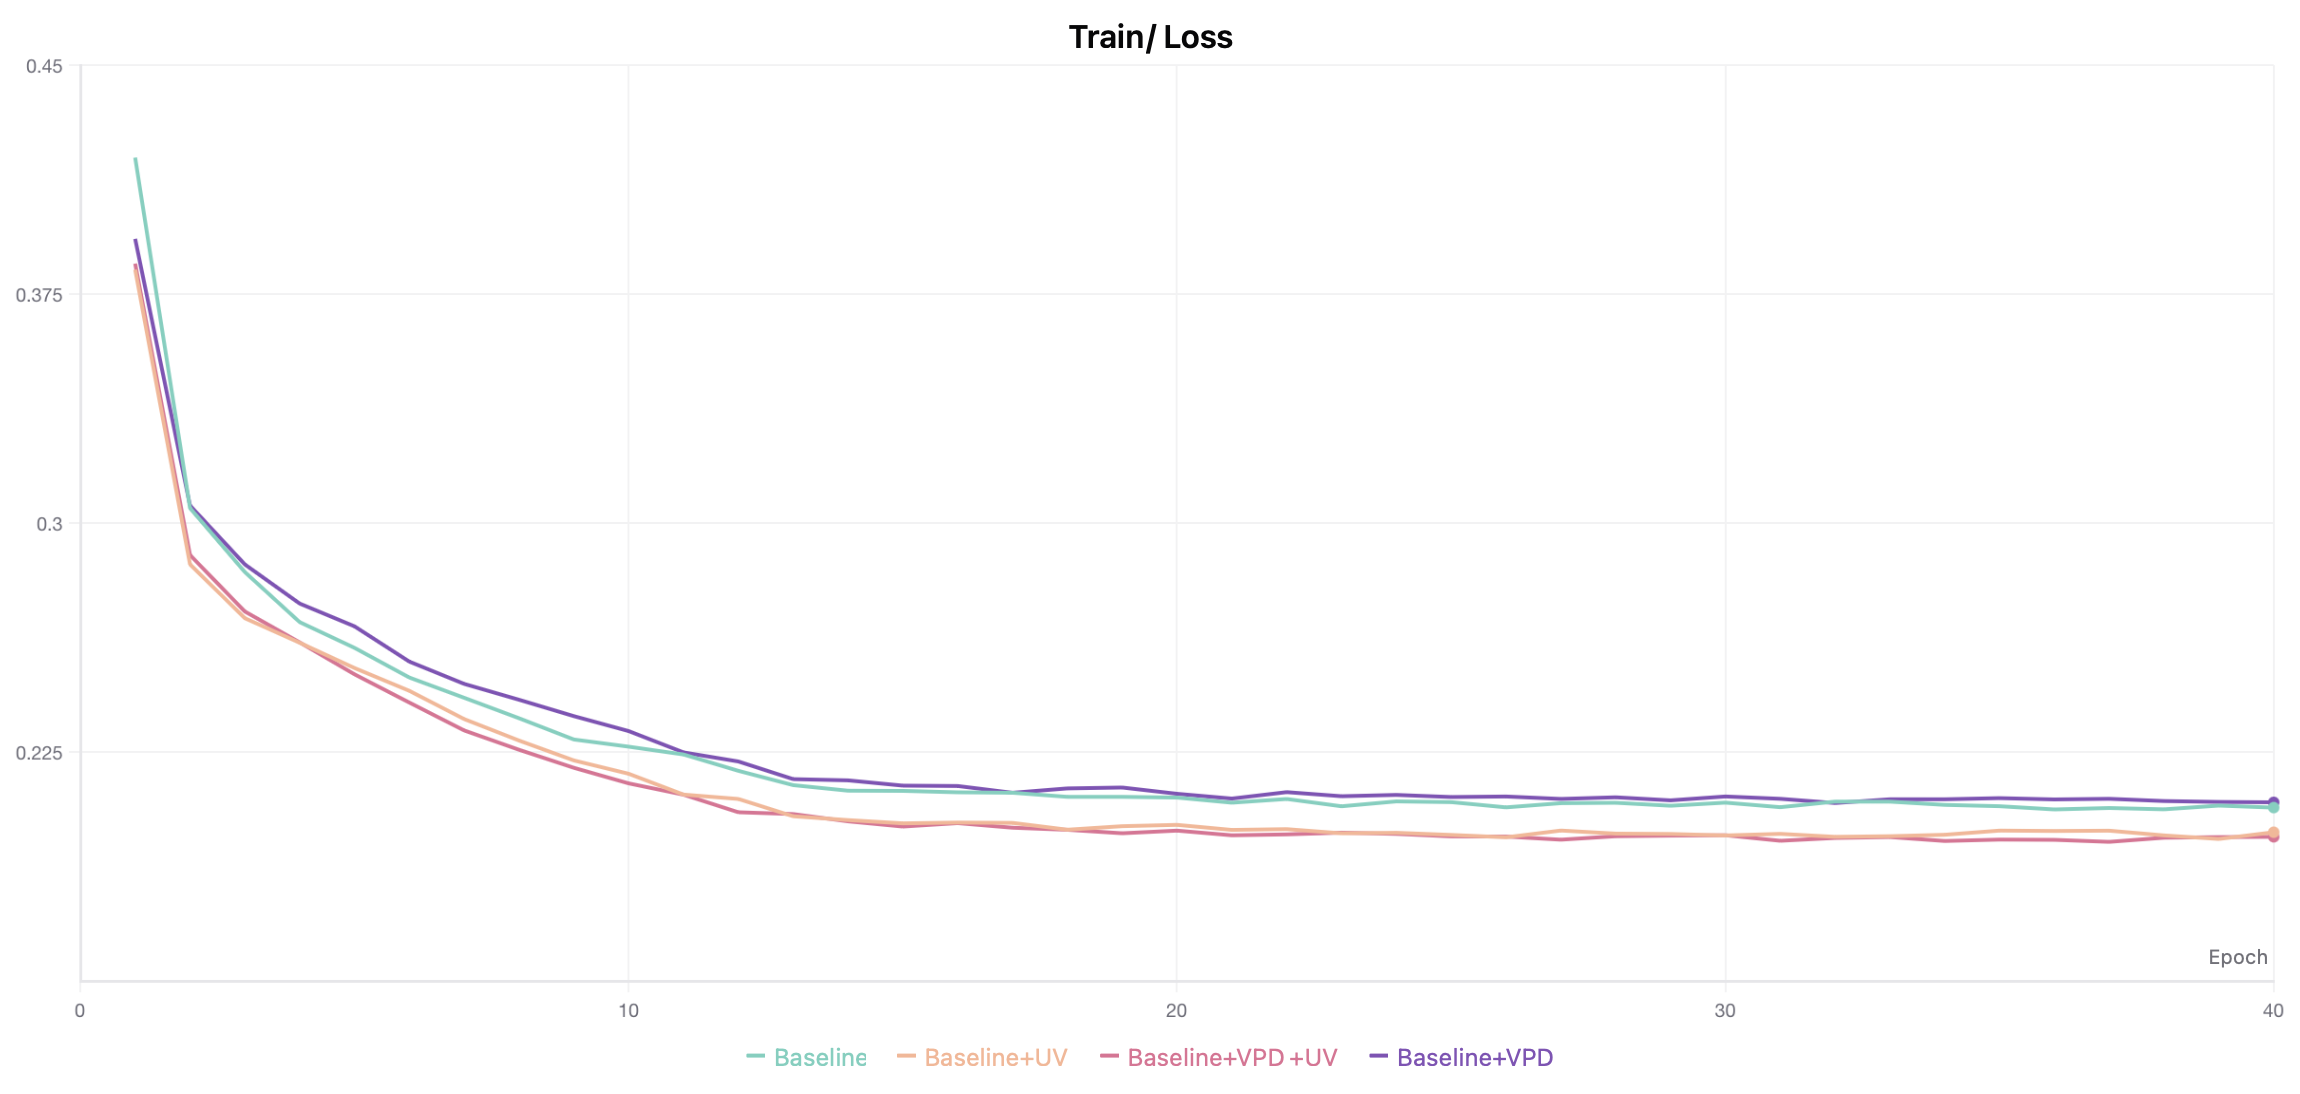
\includegraphics[width=\linewidth]{img/chap4/4-2-train-loss.png} 
        \centerline{(a) 训练集 Precision 曲线}
    \end{minipage}\hfill
    \begin{minipage}{0.48\textwidth}
        \centering
        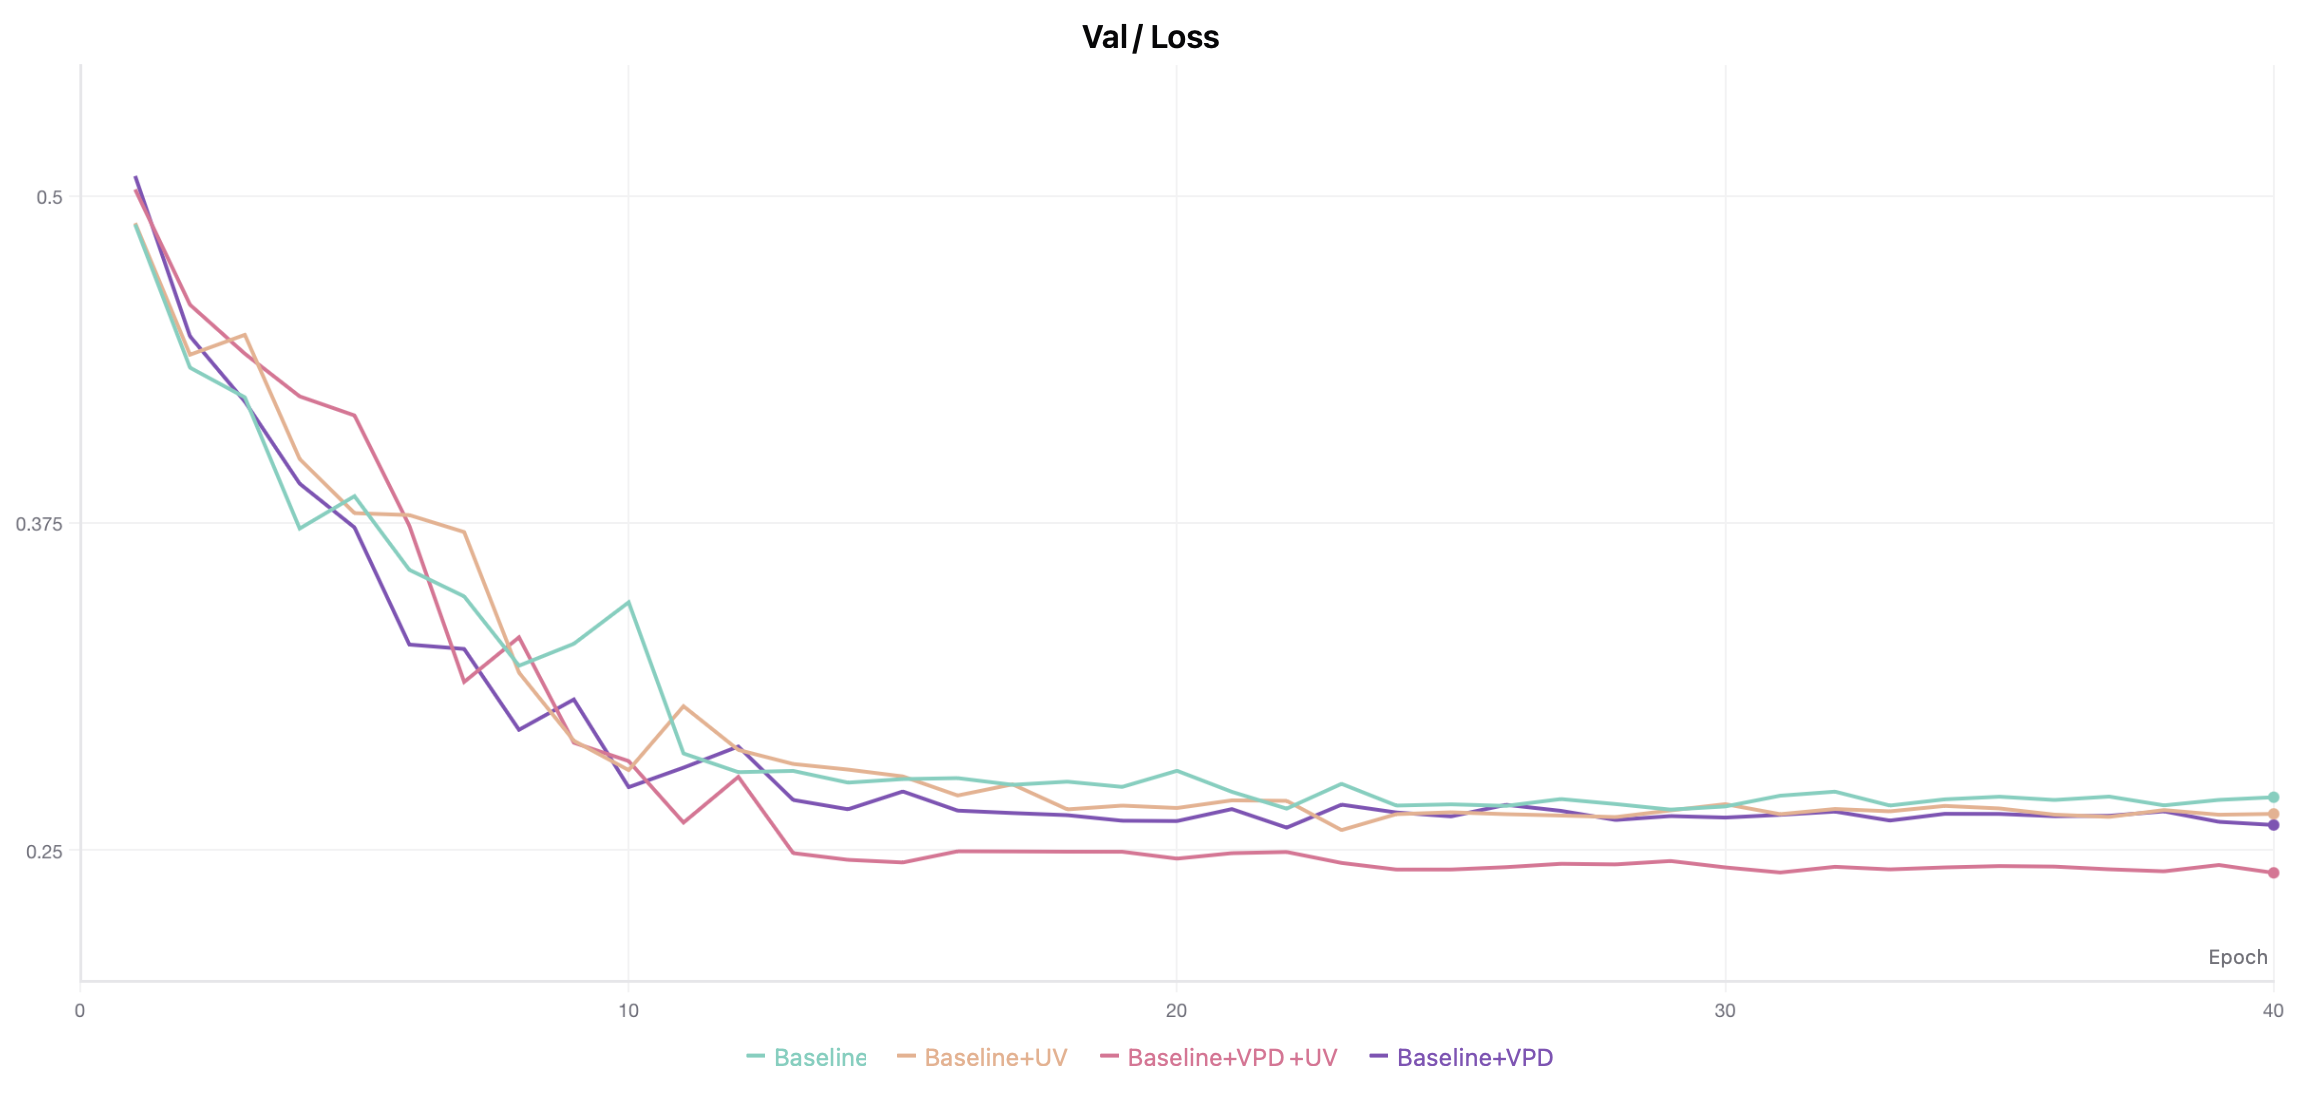
\includegraphics[width=\linewidth]{img/chap4/4-2-val-loss.png} 
        \centerline{(b) 验证集 Precision 曲线}
    \end{minipage}
    \caption{模型训练过程中的Precision曲线}
    \label{fig:4-2-train_val_precision}
\end{figure}

\section{总体预测性能对比}
\label{sec:4-3}
如表 \ref{tab:4-3-performance_comparison} 所示，本节在测试集上全面评估了模型（2D/3D Swin Transformer）与当前主流深度学习时空预测模型（LSTM, ConvLSTM, TimeSformer, 3D CNN）的定量性能。总体而言，本研究提出的融合物理信息的2D/3D Swin Transformer在总体准确率（OA）、精确率（Precision）、召回率（Recall）和核心指标 F1-Score 上均取得了全场最优表现。
\begin{table}[htbp]
    \centering
    \caption{不同深度学习模型在测试集上的定量结果，分类指标以百分比（\%）表示。}
    \label{tab:4-3-performance_comparison}
    \renewcommand{\arraystretch}{1.3} % 增加行高，提升阅读体验
    \resizebox{\textwidth}{!}{
        \begin{tabular}{lcccccc}
            \toprule
            \textbf{Algorithm} & \textbf{Config} & \textbf{Precision (↑)} & \textbf{Recall (↑)} & \textbf{F1-score (↑)} & \textbf{AUROC (↑)} & \textbf{OA (↑)} \\
            \midrule
            LSTM \cite{kondylatos2022wildfire} & -- & 73.74 & 82.17 & 77.72 & 96.53 & 93.80 \\
            ConvLSTM \cite{kondylatos2022wildfire} & -- & 82.40 & 76.75 & 79.47 & 97.12 & 94.78 \\
            TimeSformer \cite{bertasius2021space} & -- & 81.13 & 76.82 & 78.92 & 96.57 & 94.60 \\
            3D CNN \cite{loan} & -- & 82.72 & 80.98 & 81.72 & \textbf{97.15} & 95.23 \\
            \midrule
            \multirow{4}{*}{\makecell[c]{\textbf{2D/3D}\\\textbf{Swin Transformer}}}
            & Baseline & 82.41 & 82.75 & 82.58 & 96.68 & 95.41 \\
            & + VPD & 83.38 & 82.34 & 82.86 & 96.87 & 95.52 \\
            & + UV & 82.64 & \textbf{84.58} & 83.60 & 96.78 & 95.63 \\
            & + VPD + UV & \textbf{84.55} & 84.49 & \textbf{84.52} & 96.98 & \textbf{95.93} \\
            \bottomrule
        \end{tabular}
    }
\end{table}

观察基线模型数据可知，基于纯时间序列的 LSTM 模型虽然在召回率（82.17\%）上表现尚可，但其精确率仅为 73.74\%，且 F1-Score 垫底（77.72\%）。这表明缺乏空间维度交互的模型会产生大量误报。引入空间卷积的 ConvLSTM 与引入时间注意力的 TimeSformer 在精确率上有所改善，但召回率出现明显下滑。相比之下，本研究的 2D/3D Swin Transformer（Baseline）尚未引入任何物理先验，便已取得了 82.58\% 的 F1-Score，超越了所有序列和纯卷积模型。这充分证明了 Swin Transformer 的三维滑动窗口机制在捕捉火灾风险长距离时空依赖关系上的架构优越性。

在基线模型的基础上，不同物理先验信息的引入对模型性能产生了极具指向性的增益。
一方面，引入饱和水汽压差（+ VPD）后，模型的精确率（Precision）从 82.41\% 提升至 83.38\%。这从侧面印证了热力学特征重构的作用，饱和水汽压差比单纯的相对湿度更敏锐地刻画地表植被的异常脱水状态，降低了误报率。另一方面，引入风场动力学偏置（+ UV）后，模型在召回率（Recall）上实现了全场最高的 84.58\%。在野火防灾业务中，漏报的代价往往是灾难性的。风向信息的注入成功引导了模型的空间注意力向高危的下风向区域倾斜，增强了模型捕捉起火信号的能力。最终的模型（+ VPD + UV）实现了两者优势的叠加，F1-Score 达到 84.52\% 的峰值。因此，不同深度学习模型在测试集上的定量结果证明了本研究所提出模型的有效性。

